\documentclass{article}


% if you need to pass options to natbib, use, e.g.:
\PassOptionsToPackage{numbers, compress}{natbib}
% before loading neurips_2023


% ready for submission
% \usepackage{neurips_2023}



% to compile a preprint version, e.g., for submission to arXiv, add add the
% [preprint] option:
%     \usepackage[preprint]{neurips_2023}


% to compile a camera-ready version, add the [final] option, e.g.:
\usepackage[final]{neurips_2023}


% to avoid loading the natbib package, add option nonatbib:
% \usepackage[nonatbib]{neurips_2023}


% \usepackage[utf8]{inputenc} % allow utf-8 input
% \usepackage[T1]{fontenc}    % use 8-bit T1 fonts
% \usepackage{hyperref}       % hyperlinks
% \usepackage{url}            % simple URL typesetting
% \usepackage{booktabs}       % professional-quality tables
% \usepackage{amsfonts}       % blackboard math symbols
% \usepackage{nicefrac}       % compact symbols for 1/2, etc.
% \usepackage{microtype}      % microtypography
% \usepackage{xcolor}         % colors

\usepackage[utf8]{inputenc} % allow utf-8 input
\usepackage[T1]{fontenc}    % use 8-bit T1 fonts
\usepackage{hyperref}       % hyperlinks
\usepackage{url}            % simple URL typesetting
\usepackage{booktabs}       % professional-quality tables
\usepackage{amsfonts}       % blackboard math symbols
\usepackage{nicefrac}       % compact symbols for 1/2, etc.
\usepackage{microtype}      % microtypography

\usepackage{microtype}
\usepackage{graphicx}
\usepackage{subfigure}
\usepackage{booktabs} % for professional tables
\usepackage{amsmath} % For advanced math typesetting
\usepackage{amssymb} % For additional mathematical symbols

% hyperref makes hyperlinks in the resulting PDF.
% If your build breaks (sometimes temporarily if a hyperlink spans a page)
% please comment out the following usepackage line and replace
% \usepackage{icml2021} with \usepackage[nohyperref]{icml2021} above.
\usepackage{hyperref}
\usepackage[export]{adjustbox}


\title{SortFormer: Permutation Encoding for Transformer}


% The \author macro works with any number of authors. There are two commands
% used to separate the names and addresses of multiple authors: \And and \AND.
%
% Using \And between authors leaves it to LaTeX to determine where to break the
% lines. Using \AND forces a line break at that point. So, if LaTeX puts 3 of 4
% authors names on the first line, and the last on the second line, try using
% \AND instead of \And before the third author name.


\author{%
  Taejin Park \thanks{Use footnote for providing further information
    about author (webpage, alternative address)---\emph{not} for acknowledging
    funding agencies.} \\
NVIDIA, Santa Clara, CA, USA
  \texttt{taejinp@nvidia.com} \\
  % examples of more authors
  % \And
  % Coauthor \\
  % Affiliation \\
  % Address \\
  % \texttt{email} \\
  % \AND
  % Coauthor \\
  % Affiliation \\
  % Address \\
  % \texttt{email} \\
  % \And
  % Coauthor \\
  % Affiliation \\
  % Address \\
  % \texttt{email} \\
  % \And
  % Coauthor \\
  % Affiliation \\
  % Address \\
  % \texttt{email} \\
}


\begin{document}


\maketitle


\begin{abstract}
  We propose \textit{SortFormer} architecture, which is a Transformer variant that encodes permutation information into hidden states. We address the challenge of permutation invariance in processing sequential data using Transformer architectures. Despite their effectiveness in learning and generalizing across text, speech, and image data, Transformers struggle with inputs where permutations should be disregarded. This limitation often results in significant overfitting where the trained model hardly handles permutations on on the unseen datapoints. We identify that the inherent design of the original Transformer architecture contributes to this deficiency.
  % To overcome this, we introduce \textit{SortFormer}, a novel architecture that integrates a sorting mechanism to establish a unique representation for various permutations. 
  SortFormer operates by generating estimated labels at each layer, which are then sorted according to their arrival order. These sequentially ordered labels serve as a permutative encoding, guiding the Transformer model in recognizing the sequence order. Through ablation studies, we demonstrate that SortFormer exhibits reduced overfitting and enhanced generalization capabilities on unseen data sequences. Furthermore, we provide insights into the practical applicability of SortFormer in real-world scenarios. Our findings suggest that this innovative architecture holds significant promise for improving the robustness and versatility of Transformer models in handling permutation-sensitive sequential data.
  % We propose a novel but concise way to tackle the permutation problem for sequential data. While there are numerous variants of transformer architecture that can successfully learn sequential data and generalize the problem for text, speech and image. However, when it comes to inputs where the combination of permutation should be ignored, it is very challenging to let Transformer to learn only non-permutative information and generalize on the unseen data points. Thus, we show that the original Transformer architecture does not have ability to resolve permutation problem which leads to significant overfitting. We introduce a new type of architecture SortFormer which uses sorting mechanism to generate a unique representation for numerous permutations. SortFormer generates the estimated label at each layer then sort the labels in terms of arrival order. The sorted estimated labels are employed as permutative encoding to inform the order of sequence to the Transformer model. We show that the proposed architecture shows far less amount of overfitting and generalize better on unseen sequences through ablation studies. In addition, we show that the proposed architecture can be used for the real-life problems.  
\end{abstract}


\section{Introduction}
Testing autobuild 8 \\
In recent years, the large language models (LLMs) \cite{radford2019language, rao2022megatron} gained significant popularity and most of the LLMs are based on the Transformer~\cite{vaswani2017attention} architecture that is now being used for not only language modeling
as language understanding \cite{devlin2018bert, raffel2019learning}, GPT3~\cite{brown2020gpt3}. Other tasks such as image processing field also started leveraging Transformers such as image generation~\cite{parmar2018image} and image recognition with ViT~\cite{dosovitskiy2020image}. In speech recognition field, Conformer~\cite{gulati2020conformer} and Whisper~\cite{radford2023robust} successfully employed Transformer archietcture to speech-to-text (STT) tasks.

\paragraph{Transformer Variants for Efficiency}
The wide adoption of Transformer architecture also led to more efficient variants of the model such as Reformer~\cite{kitaev2019reformer}, which introduces efficient memory handling in Transformers through locality-sensitive hashing; Transformer-XL~\cite{dai2019transformer}, enhancing Transformer models for long sequence tasks with segment-level recurrence and a novel positional encoding; Performe~\cite{choromanski2020rethinking}, offering a scalable Transformer variant with the new attention mechanism for processing long sequences efficiently; Longformer~\cite{beltagy2020longformer}, designed for longer texts with a modified attention mechanism that combines sliding window and global attention for tasks like document classification and question answering; SegFormer~\cite{xie2021segformer}, an approach for semantic segmentation combining a hierarchical Transformer encoder with a lightweight MLP decoder; and RoFormer\cite{su2023roformer}, which enhances Transformer models with a rotational position encoding scheme for improved performance in various natural language processing tasks. These variants showcase significant advancements in handling long sequences, improving memory efficiency, and extending the applicability of Transformer models in various domains, including text and image processing.

\paragraph{Problem that SortFormer solves}
% In the application for language modeling in \cite{radford2019language} or speech recognition \cite{radford2023robust}, input sequence $\mathbf{X}$ 

% The input sequence \( \mathbf{X} \) can be represented as:
% \begin{align}
%   \mathbf{X} & = \{\mathbf{x}_1, \mathbf{x}_2, \ldots, \mathbf{x}_T\} \\
%   \mathbf{Y} & = \{\mathbf{y}_1, \mathbf{y}_2, \ldots, \mathbf{y}_T\}
% \end{align}

% where each \( \mathbf{x}_i \) is a vector representing a token or embedding in the input sequence.
% Output Sequence
% The output sequence \( \mathbf{Y} \) can be represented as:
% where each \( \mathbf{y}_j \) is a vector representing a token in the output sequence.

We propose a model designed for the simultaneous estimation of class presences from a sequence of input tokens.
Consider a set of frame-wise \( F \)-dimensional embedding vectors
$ \{ \mathbf{x}_t \}_{t=1}^T $, where $ \mathbf{x}_t \in \mathbb{R}^D, t = 1, 2, \ldots, T $, representing the frame index.
Given the input sequence, the model is expected to generate the estimated sequence $\{ \mathbf{y}_t \}_{t=1}^T$, where $ \mathbf{y}_t \in \mathbb{R}^K, t = 1, 2, \ldots, T $.
SortFormer is tasked with estimating the class presences \( \left\{\mathbf{y}_t\right\}_{t=1}^T \). In this context, $\mathbf{y}_t =$ {\small $\left[y_{1, t}, y_{2, t}, \ldots, y_{K, t}\right]^{\top}$}
denotes the class presences of \( K \) classes at time \( t \). SortFormer operates under the assumption that $ y_{k, t} $ is conditionally independent given the embedding vectors (features). This assumption is formalized as:

\begin{align}
  P\left(\mathbf{y}_1, \ldots, \mathbf{y}_T \mid \mathbf{x}_1, \ldots, \mathbf{x}_T\right) = \prod_{k=1}^K\prod_{t=1}^T  P\left(y_{k, t} \mid \mathbf{x}_1, \ldots, \mathbf{x}_T\right).
\end{align}

Under this framework, the task at hand is construed as a multi-label classification problem, which is amenable to modeling via a neural network, denoted as  $f_{\Theta}$. The model is defined as:

\begin{align}
  \left(\mathbf{p}_1, \ldots, \mathbf{p}_T\right) = f_{\Theta}\left(\mathbf{x}_1, \ldots, \mathbf{x}_T\right),
\end{align}

where \( \mathbf{p}_t = \left[p_{1, t}, \ldots, p_{K, t}\right]^{\top} \in (0,1)^S \) represents the posterior probabilities of the presences of \( S \) classes at frame index \( t \) and f represents
the Sortformer model with parameter.
Each \( y_{k, t} \) is defined as follows depending on the value of \( p_{k, t} \):
\begin{align}
  y_{k,t} = 
  \begin{cases} 
      1 & \text{if } p_{k,t} > 0.5 \\
      0 & \text{if } p_{k,t} \leq 0.5 
  \end{cases}
\end{align}

The estimation of class presences $\left\{\hat{\mathbf{y}}_t\right\}_{t=1}^T$ is given by:

\begin{align}
  (\hat{\mathbf{y}}_1, \ldots, \hat{\mathbf{y}}_T) & = \underset{\mathbf{y}_k \in \mathbf{Y}}{\arg\max} \big\{ P\left(\mathbf{y}_1, \ldots, \mathbf{y}_T \mid \mathbf{x}_1, \ldots, \mathbf{x}_T\right) \big\},
  \label{eq:sortformer_vector}
\end{align}
The equation \ref{eq:sortformer_vector} can be rewritten in matrix form by concatenating the vectors $ \mathbf{X} = [ \mathbf{x}_1 \mathbf{x}_2 \ldots, \mathbf{x}_T ] $,
where each column of $\mathbf{Y}$ represents the class presences at time $t$, $ \mathbf{Y} = [\mathbf{y}_1 \, \mathbf{y}_2 \, \ldots \, \mathbf{y}_T]$.
In the simplest form, the model can be represented as:
\begin{align}
\mathbf{Y} = f_{\Theta}\left(\mathbf{X}\right),
\end{align}
where \( \mathbf{X} \in \mathbb{R}^{D \times T} \) is the input sequence and \( \mathbf{Y} \in \mathbb{R}^{K \times T} \) is a binary matrix contains an output sequence. 
The most crucial part of the problem is the number of none-zero rows in the output sequence \( \mathbf{Y} \) is determined by the estimation from the model based on the input sequence \( \mathbf{X} \).
This 

\paragraph{Permutation Invariance in Neural Network}
Problem

\section{Prior Works}

\paragraph{clustering}
There have been numerous studies on making Transformer to perceive longer context, model compressing for memory efficiency and sparse models. However, there have been limited number of published work regarding general-purpose transformer variants which can handle permutation

The most closest previous study to our work is Set-Transformer \cite{lee2019set},
\paragraph{permutation invairant loss}

\paragraph{clustering}


\section{Permutation Invariance for Transformers}



% \begin{figure}
%     \centering
%     \subfigure[]{ \centering
%     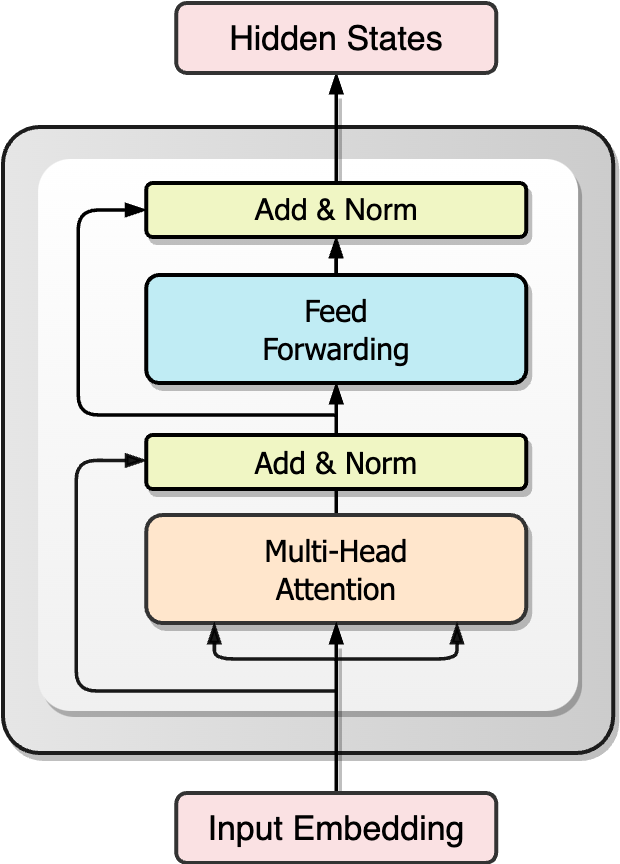
\includegraphics[width=0.2\textwidth, left]{pics/TransformerEncoder.drawio.png}} 
%     \subfigure[]{  \centering
%     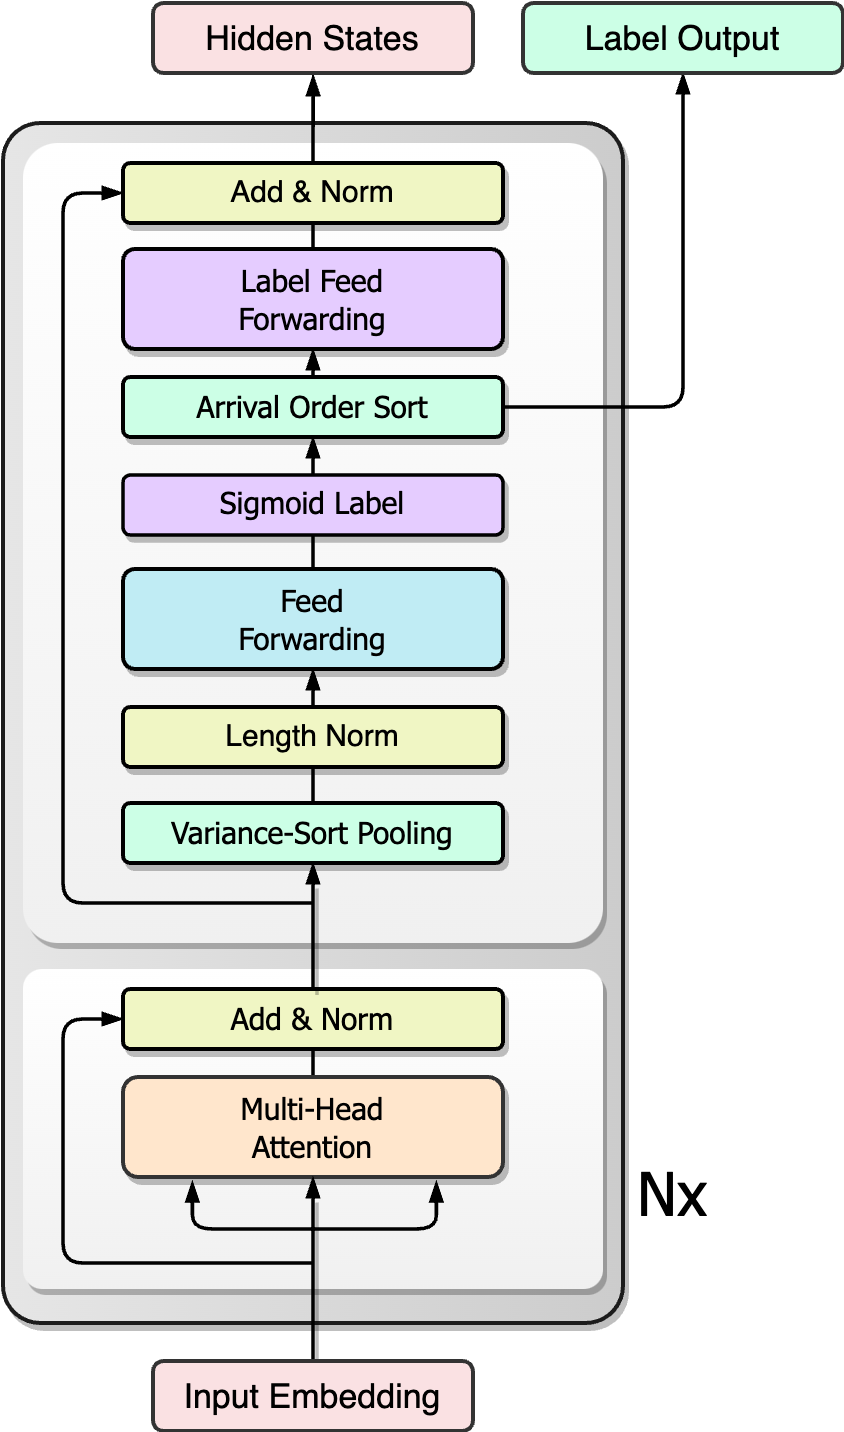
\includegraphics[width=0.24\textwidth, center]{pics/SortFormerEncoder.png}} 
%     \subfigure[]{  \centering
%     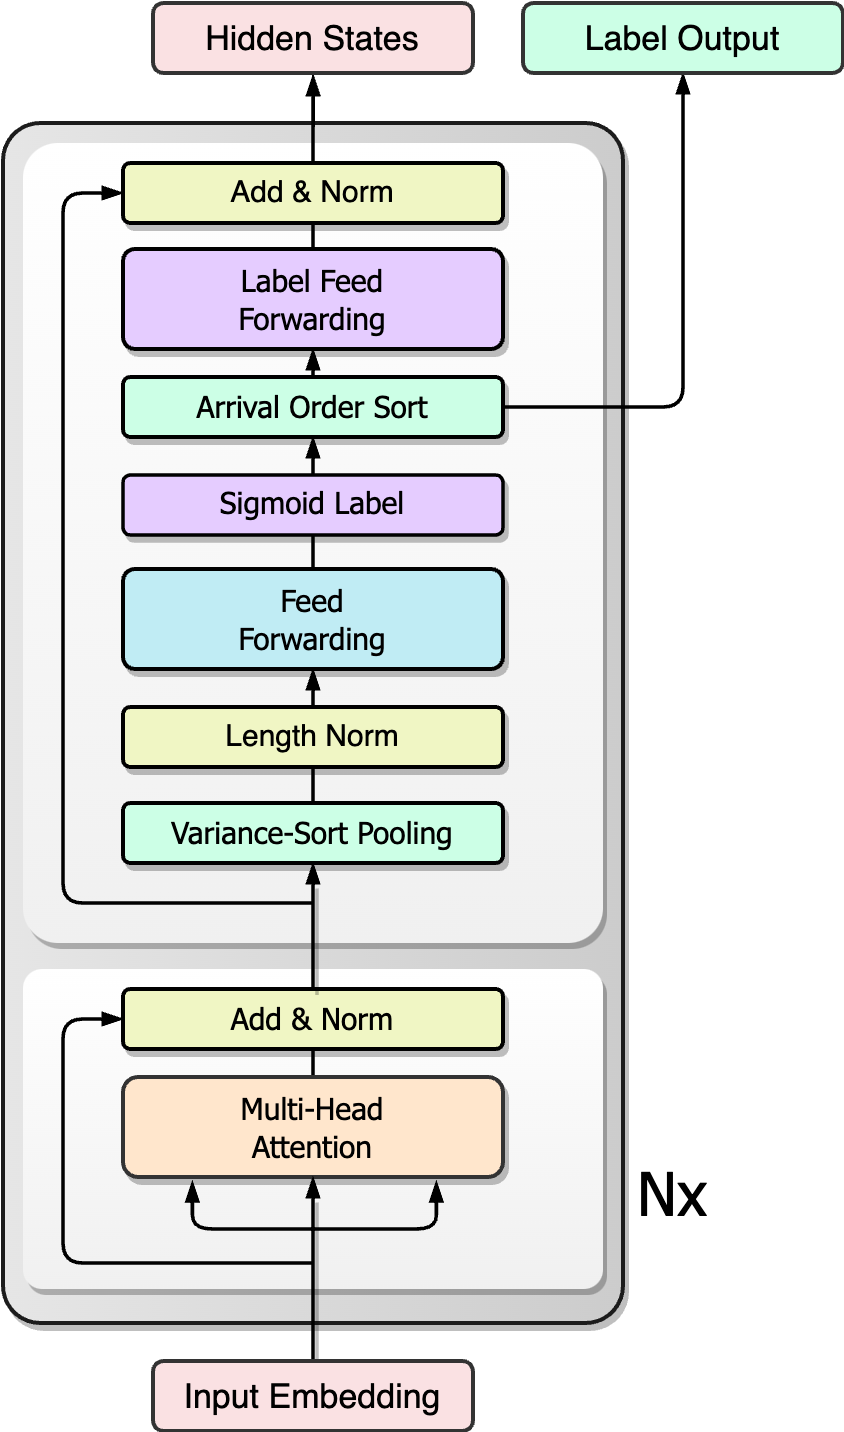
\includegraphics[width=0.24\textwidth, right]{pics/SortFormerEncoder.png}}
%     % \subfigure[]{\includegraphics[width=0.24\textwidth]{monalisa.jpg}}
%     % \caption{(a) blah (b) blah (c) blah (d) blah}
%     \label{fig:foobar}
% \end{figure}

\begin{figure}[ht]
  % \begin{subfigure}[width=0.5\textwidth]{}
  \begin{minipage}[b]{0.33\textwidth}
    \centering
    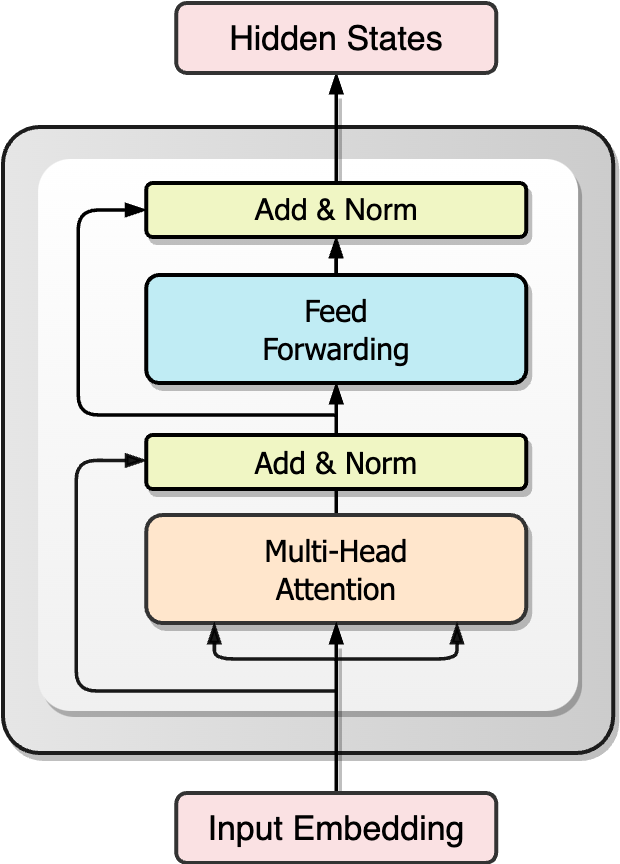
\includegraphics[width=0.73\linewidth]{pics/TransformerEncoder.drawio.png}
    \caption{Caption1}
    \label{fig:subim1}
  \end{minipage}
  \begin{minipage}[b]{0.33\textwidth}
    \centering
    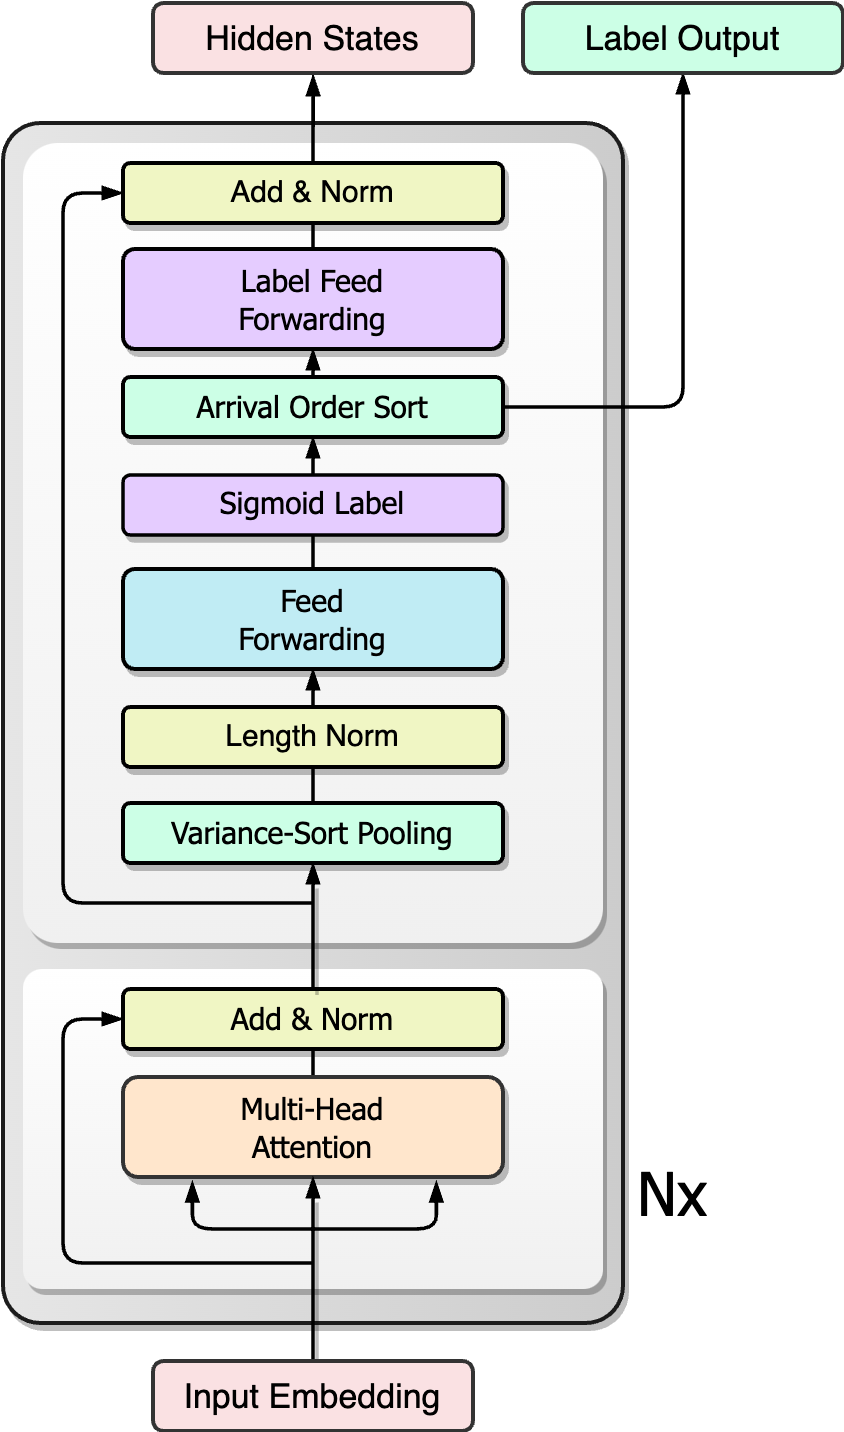
\includegraphics[width=0.9\linewidth]{pics/SortFormerEncoder.png}
    \caption{Caption 2}
    \label{fig:subim2}
  \end{minipage}
  \begin{minipage}[b]{0.33\textwidth}
    \centering
    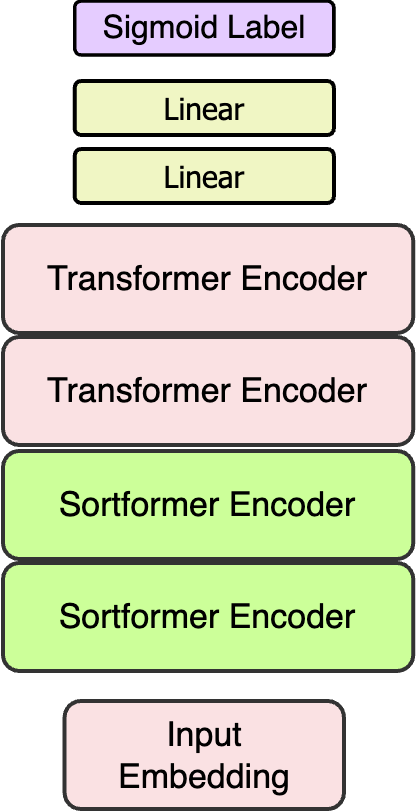
\includegraphics[width=0.5\linewidth]{pics/SortFormer_example.drawio.png}
    \caption{Caption 3}
    \label{fig:subim3}
  \end{minipage}
\end{figure}


\subsection{Copied and Pasted from a Paper}
\cite{bloem2018neural}. This section is fo
Let $Y \in \mathcal{Y}$ be some random variable of interest, to be predicted from $\mathbf{X}_n$. Permutation invariance of the conditional distribution $P_{Y \mid \mathbf{x}_n}$ of $Y$ given $\mathbf{X}_n$ is defined as follows.

Definition 1. The conditional distribution $P_{Y \mid \mathbf{X}_n}$ of $Y$ given $\mathbf{X}_n$ is $\mathbb{S}_n$-invariant if for all $B \in \mathcal{B}(\mathcal{Y})$ and $\pi \in \mathbb{S}_n$,

\begin{align}
  P_{Y \mid \mathbf{X}_n}\left[Y \in B \mid \pi \cdot \mathbf{X}_n\right]=P_{Y \mid \mathbf{X}_n}\left[Y \in B \mid \mathbf{X}_n\right] \quad \text { a.s. }-P_{\mathbf{X}_n} .
\end{align}

Together with exchangeability of $P_{\mathbf{X}_n}$, conditional invariance implies the joint equality $\left(\pi \cdot \mathbf{X}_n, Y\right) \stackrel{\text { d }}{=}\left(\mathbf{X}_n, Y\right)$ for all $\pi \in \mathbb{S}_n$.

In the neural networks literature, equivariance plays a key role in the hidden layers of invariant deterministic neural networks $[2,8,6]$. As we show in Section 2, the following adaptation to random variables plays the same role in $\mathbb{S}_n$-invariant stochastic neural networks.

Definition 2. Let $\mathbf{Y}_n \in \mathcal{Y}^n$ be a random $\mathcal{Y}$-valued sequence. The conditional distribution $P_{\mathbf{Y}_n \mid \mathbf{x}_n}$ of $\mathbf{Y}_n$ given $\mathbf{X}_n$ is $\mathbb{S}_n$-equivariant if for all $B \in \mathcal{B}\left(\mathcal{Y}^n\right)$ and $\pi \in \mathbb{S}_n$,

\begin{align}
  P_{\mathbf{Y}_n \mid \mathbf{X}_n}\left[\pi \cdot \mathbf{Y}_n \in B \mid \pi \cdot \mathbf{X}_n\right]=P_{\mathbf{Y}_n \mid \mathbf{X}_n}\left[\mathbf{Y}_n \in B \mid \mathbf{X}_n\right] \quad \text { a.s. }-P_{\mathbf{X}_n} .
\end{align}

Together with exchangeability of $P_{\mathbf{X}_n}$, conditional invariance implies the joint equality $\left(\pi \cdot \mathbf{X}_n, \pi \cdot \mathbf{Y}_n\right) \stackrel{\mathrm{d}}{=}\left(\mathbf{X}_n, \mathbf{Y}_n\right)$ for all $\pi \in \mathbb{S}_n$


\section{Submission of papers to NeurIPS 2023}


Please \cite{vaswani2017attention} read the instructions below carefully and follow them faithfully. \textbf{Important:} This year the checklist will be submitted separately from the main paper in OpenReview, please review it well ahead of the submission deadline: \url{https://neurips.cc/public/guides/PaperChecklist}.


\subsection{Style}


Papers to be submitted to NeurIPS 2023 must be prepared according to the
instructions presented here. Papers may only be up to {\bf nine} pages long,
including figures. Additional pages \emph{containing only acknowledgments and
  references} are allowed. Papers that exceed the page limit will not be
reviewed, or in any other way considered for presentation at the conference.


The margins in 2023 are the same as those in previous years.


Authors are required to use the NeurIPS \LaTeX{} style files obtainable at the
NeurIPS website as indicated below. Please make sure you use the current files
and not previous versions. Tweaking the style files may be grounds for
rejection.


\subsection{Retrieval of style files}


The style files for NeurIPS and other conference information are available on
the website at
\begin{center}
  \url{http://www.neurips.cc/}
\end{center}
The file \verb+neurips_2023.pdf+ contains these instructions and illustrates the
various formatting requirements your NeurIPS paper must satisfy.


The only supported style file for NeurIPS 2023 is \verb+neurips_2023.sty+,
rewritten for \LaTeXe{}.  \textbf{Previous style files for \LaTeX{} 2.09,
  Microsoft Word, and RTF are no longer supported!}


The \LaTeX{} style file contains three optional arguments: \verb+final+, which
creates a camera-ready copy, \verb+preprint+, which creates a preprint for
submission to, e.g., arXiv, and \verb+nonatbib+, which will not load the
\verb+natbib+ package for you in case of package clash.


\paragraph{Preprint option}
If you wish to post a preprint of your work online, e.g., on arXiv, using the
NeurIPS style, please use the \verb+preprint+ option. This will create a
nonanonymized version of your work with the text ``Preprint. Work in progress.''
in the footer. This version may be distributed as you see fit, as long as you do not say which conference it was submitted to. Please \textbf{do
  not} use the \verb+final+ option, which should \textbf{only} be used for
papers accepted to NeurIPS.


At submission time, please omit the \verb+final+ and \verb+preprint+
options. This will anonymize your submission and add line numbers to aid
review. Please do \emph{not} refer to these line numbers in your paper as they
will be removed during generation of camera-ready copies.


The file \verb+neurips_2023.tex+ may be used as a ``shell'' for writing your
paper. All you have to do is replace the author, title, abstract, and text of
the paper with your own.


The formatting instructions contained in these style files are summarized in
Sections \ref{gen_inst}, \ref{headings}, and \ref{others} below.


\section{General formatting instructions}
\label{gen_inst}


The text must be confined within a rectangle 5.5~inches (33~picas) wide and
9~inches (54~picas) long. The left margin is 1.5~inch (9~picas).  Use 10~point
type with a vertical spacing (leading) of 11~points.  Times New Roman is the
preferred typeface throughout, and will be selected for you by default.
Paragraphs are separated by \nicefrac{1}{2}~line space (5.5 points), with no
indentation.


The paper title should be 17~point, initial caps/lower case, bold, centered
between two horizontal rules. The top rule should be 4~points thick and the
bottom rule should be 1~point thick. Allow \nicefrac{1}{4}~inch space above and
below the title to rules. All pages should start at 1~inch (6~picas) from the
top of the page.


For the final version, authors' names are set in boldface, and each name is
centered above the corresponding address. The lead author's name is to be listed
first (left-most), and the co-authors' names (if different address) are set to
follow. If there is only one co-author, list both author and co-author side by
side.


Please pay special attention to the instructions in Section \ref{others}
regarding figures, tables, acknowledgments, and references.


\section{Headings: first level}
\label{headings}


All headings should be lower case (except for first word and proper nouns),
flush left, and bold.


First-level headings should be in 12-point type.


\subsection{Headings: second level}


Second-level headings should be in 10-point type.


\subsubsection{Headings: third level}


Third-level headings should be in 10-point type.


\paragraph{Paragraphs}


There is also a \verb+\paragraph+ command available, which sets the heading in
bold, flush left, and inline with the text, with the heading followed by 1\,em
of space.


\section{Citations, figures, tables, references}
\label{others}


These instructions apply to everyone.


\subsection{Citations within the text}


The \verb+natbib+ package will be loaded for you by default.  Citations may be
author/year or numeric, as long as you maintain internal consistency.  As to the
format of the references themselves, any style is acceptable as long as it is
used consistently.


The documentation for \verb+natbib+ may be found at
\begin{center}
  \url{http://mirrors.ctan.org/macros/latex/contrib/natbib/natnotes.pdf}
\end{center}
Of note is the command \verb+\citet+, which produces citations appropriate for
use in inline text.  For example,
\begin{verbatim}
   \citet{hasselmo} investigated\dots
\end{verbatim}
produces
\begin{quote}
  Hasselmo, et al.\ (1995) investigated\dots
\end{quote}


If you wish to load the \verb+natbib+ package with options, you may add the
following before loading the \verb+neurips_2023+ package:
\begin{verbatim}
   \PassOptionsToPackage{options}{natbib}
\end{verbatim}


If \verb+natbib+ clashes with another package you load, you can add the optional
argument \verb+nonatbib+ when loading the style file:
\begin{verbatim}
   \usepackage[nonatbib]{neurips_2023}
\end{verbatim}


As submission is double blind, refer to your own published work in the third
person. That is, use ``In the previous work of Jones et al.\ [4],'' not ``In our
previous work [4].'' If you cite your other papers that are not widely available
(e.g., a journal paper under review), use anonymous author names in the
citation, e.g., an author of the form ``A.\ Anonymous'' and include a copy of the anonymized paper in the supplementary material.


\subsection{Footnotes}


Footnotes should be used sparingly.  If you do require a footnote, indicate
footnotes with a number\footnote{Sample of the first footnote.} in the
text. Place the footnotes at the bottom of the page on which they appear.
Precede the footnote with a horizontal rule of 2~inches (12~picas).


Note that footnotes are properly typeset \emph{after} punctuation
marks.\footnote{As in this example.}


\subsection{Figures}


\begin{figure}
  \centering
  \fbox{\rule[-.5cm]{0cm}{4cm} \rule[-.5cm]{4cm}{0cm}}
  \caption{Sample figure caption.}
\end{figure}


All artwork must be neat, clean, and legible. Lines should be dark enough for
purposes of reproduction. The figure number and caption always appear after the
figure. Place one line space before the figure caption and one line space after
the figure. The figure caption should be lower case (except for first word and
proper nouns); figures are numbered consecutively.


You may use color figures.  However, it is best for the figure captions and the
paper body to be legible if the paper is printed in either black/white or in
color.


\subsection{Tables}


All tables must be centered, neat, clean and legible.  The table number and
title always appear before the table.  See Table~\ref{sample-table}.


Place one line space before the table title, one line space after the
table title, and one line space after the table. The table title must
be lower case (except for first word and proper nouns); tables are
numbered consecutively.


Note that publication-quality tables \emph{do not contain vertical rules.} We
strongly suggest the use of the \verb+booktabs+ package, which allows for
typesetting high-quality, professional tables:
\begin{center}
  \url{https://www.ctan.org/pkg/booktabs}
\end{center}
This package was used to typeset Table~\ref{sample-table}.


\begin{table}
  \caption{Sample table title}
  \label{sample-table}
  \centering
  \begin{tabular}{lll}
    \toprule
    \multicolumn{2}{c}{Part}                   \\
    \cmidrule(r){1-2}
    Name     & Description     & Size ($\mu$m) \\
    \midrule
    Dendrite & Input terminal  & $\sim$100     \\
    Axon     & Output terminal & $\sim$10      \\
    Soma     & Cell body       & up to $10^6$  \\
    \bottomrule
  \end{tabular}
\end{table}

\subsection{Math}
Note that display math in bare TeX commands will not create correct line numbers for submission. Please use LaTeX (or AMSTeX) commands for unnumbered display math. (You really shouldn't be using \$\$ anyway; see \url{https://tex.stackexchange.com/questions/503/why-is-preferable-to} and \url{https://tex.stackexchange.com/questions/40492/what-are-the-differences-between-align-equation-and-displaymath} for more information.)

\subsection{Final instructions}

Do not change any aspects of the formatting parameters in the style files.  In
particular, do not modify the width or length of the rectangle the text should
fit into, and do not change font sizes (except perhaps in the
\textbf{References} section; see below). Please note that pages should be
numbered.


\section{Preparing PDF files}


Please prepare submission files with paper size ``US Letter,'' and not, for
example, ``A4.''


Fonts were the main cause of problems in the past years. Your PDF file must only
contain Type 1 or Embedded TrueType fonts. Here are a few instructions to
achieve this.


\begin{itemize}


  \item You should directly generate PDF files using \verb+pdflatex+.


  \item You can check which fonts a PDF files uses.  In Acrobat Reader, select the
        menu Files$>$Document Properties$>$Fonts and select Show All Fonts. You can
        also use the program \verb+pdffonts+ which comes with \verb+xpdf+ and is
        available out-of-the-box on most Linux machines.


  \item \verb+xfig+ "patterned" shapes are implemented with bitmap fonts.  Use
        "solid" shapes instead.


  \item The \verb+\bbold+ package almost always uses bitmap fonts.  You should use
        the equivalent AMS Fonts:
        \begin{verbatim}
   \usepackage{amsfonts}
\end{verbatim}
        followed by, e.g., \verb+\mathbb{R}+, \verb+\mathbb{N}+, or \verb+\mathbb{C}+
        for $\mathbb{R}$, $\mathbb{N}$ or $\mathbb{C}$.  You can also use the following
        workaround for reals, natural and complex:
        \begin{verbatim}
   \newcommand{\RR}{I\!\!R} %real numbers
   \newcommand{\Nat}{I\!\!N} %natural numbers
   \newcommand{\CC}{I\!\!\!\!C} %complex numbers
\end{verbatim}
        Note that \verb+amsfonts+ is automatically loaded by the \verb+amssymb+ package.


\end{itemize}


If your file contains type 3 fonts or non embedded TrueType fonts, we will ask
you to fix it.


\subsection{Margins in \LaTeX{}}


Most of the margin problems come from figures positioned by hand using
\verb+\special+ or other commands. We suggest using the command
\verb+\includegraphics+ from the \verb+graphicx+ package. Always specify the
figure width as a multiple of the line width as in the example below:
\begin{verbatim}
   \usepackage[pdftex]{graphicx} ...
   \includegraphics[width=0.8\linewidth]{myfile.pdf}
\end{verbatim}
See Section 4.4 in the graphics bundle documentation
(\url{http://mirrors.ctan.org/macros/latex/required/graphics/grfguide.pdf})


A number of width problems arise when \LaTeX{} cannot properly hyphenate a
line. Please give LaTeX hyphenation hints using the \verb+\-+ command when
necessary.


\begin{ack}
  Use unnumbered first level headings for the acknowledgments. All acknowledgments
  go at the end of the paper before the list of references. Moreover, you are required to declare
  funding (financial activities supporting the submitted work) and competing interests (related financial activities outside the submitted work).
  More information about this disclosure can be found at: \url{https://neurips.cc/Conferences/2023/PaperInformation/FundingDisclosure}.


  Do {\bf not} include this section in the anonymized submission, only in the final paper. You can use the \texttt{ack} environment provided in the style file to autmoatically hide this section in the anonymized submission.
\end{ack}



\section{Supplementary Material}

Authors may wish to optionally include extra information (complete proofs, additional experiments and plots) in the appendix. All such materials should be part of the supplemental material (submitted separately) and should NOT be included in the main submission.


\section*{References}


References follow the acknowledgments in the camera-ready paper. Use unnumbered first-level heading for
the references. Any choice of citation style is acceptable as long as you are
consistent. It is permissible to reduce the font size to \verb+small+ (9 point)
when listing the references.
Note that the Reference section does not count towards the page limit.
\medskip

\bibliography{sortformer}
\bibliographystyle{plainnat}
% \bibliographystyle{}


% {
% \small


% [1] Alexander, J.A.\ \& Mozer, M.C.\ (1995) Template-based algorithms for
% connectionist rule extraction. In G.\ Tesauro, D.S.\ Touretzky and T.K.\ Leen
% (eds.), {\it Advances in Neural Information Processing Systems 7},
% pp.\ 609--616. Cambridge, MA: MIT Press.


% [2] Bower, J.M.\ \& Beeman, D.\ (1995) {\it The Book of GENESIS: Exploring
%   Realistic Neural Models with the GEneral NEural SImulation System.}  New York:
% TELOS/Springer--Verlag.


% [3] Hasselmo, M.E., Schnell, E.\ \& Barkai, E.\ (1995) Dynamics of learning and
% recall at excitatory recurrent synapses and cholinergic modulation in rat
% hippocampal region CA3. {\it Journal of Neuroscience} {\bf 15}(7):5249-5262.
% }

%%%%%%%%%%%%%%%%%%%%%%%%%%%%%%%%%%%%%%%%%%%%%%%%%%%%%%%%%%%%


\end{document}